% !TEX root = ../BookTemplate.tex
%%%%%%%%%%%%%%%%%%%%%%%%%%%%%%%%%%%%%%%%%%%%%%%%%%%%%%%%%%%%%%%%%%%%%%%%%%%%%%%%%%
\chapter{Methodology}
\label{ch:methodology}

\section{Methodology Overview}

\begin{figure}[htbp]
    \centering
    \includegraphics[width=1\textwidth]{Images/methodology_flowchart.png}
    \caption{Methodology flowchart showing the six-stage research pipeline.}
    \label{fig:methodology_flowchart}
\end{figure}

The overall methodology of this project followed a six-stage pipeline, progressing from primary data collection through to a deployable Early Warning System (EWS) dashboard prototype, as illustrated in Fig.~\ref{fig:methodology_flowchart}. The stages were: (1) Data Collection, (2) Data Preprocessing, (3) Exploratory Data Analysis (EDA), (4) Feature Engineering, (5) Predictive Modelling, and (6) UI Dashboard Development. Each stage informed the next, with findings from the EDA shaping feature engineering decisions, student segmentation profiles, and model selection criteria. A parallel Student Segmentation module (K-Means Clustering) was applied after Feature Engineering to generate interpretable student risk profiles that complement the binary classifier outputs in the final dashboard.

%%============================================================================
\section{Data Collection}
\label{sec:data_collection}

\subsection{Data Source and Collection Instrument}
This study utilizes primary survey data collected from students across multiple educational institutions and provinces in Cambodia. Recognizing the limitations of administrative records and learning management system (LMS) logs in offline, rural classroom contexts, the research employs a structured digital questionnaire designed to capture the multidimensional determinants of student attrition. The survey instrument was distributed via Google Forms in both Khmer and English to maximize accessibility across student cohorts with differing language proficiencies.

The questionnaire systematically elicits information across five core domains: (i)~demographic characteristics, (ii)~academic engagement patterns, (iii)~socioeconomic background, (iv)~familial and community support structures, and (v)~self-reported attitudes toward school continuation. Operationalized variables include both objective indicators---such as attendance frequency, monthly academic performance, distance to school, and primary transportation mode---and contextual factors such as parental education level, household income, living arrangements, and perceived access to external educational assistance. The target variable, \texttt{thought\_dropout}, is encoded as a binary indicator reflecting at-risk ($1$) versus non-at-risk ($0$) status.

\subsection{Features Collected}
\label{subsec:features}
The survey instrument captured 16 features spanning five thematic categories. Table~\ref{tab:dataset_summary} provides the full coding scheme and variable types for each feature. A summary of the five categories is as follows:
\begin{itemize}
    \item \textbf{Demographics}: gender, age, province of origin, standardized study level (grade)
    \item \textbf{Living Situation}: who the student lives with during the school term, distance from home to school, and primary transport method
    \item \textbf{Socioeconomic Factors}: subjective family income level, parental education level, and whether the student works to financially support their family
    \item \textbf{Academic Performance}: weekly school attendance days, self-reported absence frequency, and average monthly study score bracket
    \item \textbf{Psychosocial and Support Factors}: access to external educational support (NGOs, scholarships, or family aid), and the binary target variable \texttt{thought\_dropout}
\end{itemize}

\subsection{Dataset Summary}
\label{subsec:dataset_summary}
Table~\ref{tab:dataset_summary} summarizes the coding, variable type, and descriptive characteristics of the raw survey features. The raw survey yielded 556 initial responses. To establish a homogeneous cohort focused on the critical lower secondary school dropout window (Grades 7--12, where student attrition rates are highest in Cambodia), the dataset was cleaned through three filtering steps: removing university and post-graduate students ($N=130$), correcting or removing records with invalid age entries ($N=4$), and dropping incomplete or exact duplicate rows ($N=22$). This yielded a final analytical sample of $N=400$ student profiles.

\begin{table}[!htbp]
    \centering
    \caption{Summary of Survey Variables, Variable Types, and Coding Schemes}
    \label{tab:dataset_summary}
    \small
    \begin{tabular}{llll}
        \toprule
        \textbf{Category} & \textbf{Feature} & \textbf{Type} & \textbf{Coding / Values} \\
        \midrule
        Demographics & \texttt{gender}              & Nominal   & Female (0), Male (1), Other (2) \\
                     & \texttt{age}                 & Numerical & Integer years (range: 12--27) \\
                     & \texttt{province}            & Nominal   & Kampong Cham, Kampot, Battambang, etc. \\
                     & \texttt{study\_level}        & Ordinal   & Grade 7 to Grade 12 \\
        \midrule
        Living       & \texttt{living\_with}        & Nominal   & Both parents (0), Single/Relatives (1) \\
                     & \texttt{distance}            & Ordinal   & $<$1\,km (1), 1--5\,km (2), $>$5\,km (3) \\
                     & \texttt{transport}           & Nominal   & Walk (0), Bicycle (1), Motorbike (2), Car (3) \\
        \midrule
        Socioeconomic & \texttt{family\_income}      & Binary    & Low (0), Medium (1) \\
                      & \texttt{parental\_education} & Ordinal   & None (0) to Higher (4) \\
                      & \texttt{work\_support}       & Binary    & Does not work (0), Works (1) \\
        \midrule
        Academic     & \texttt{attendance}          & Ordinal   & 0--2\,d/wk (0), 3--4\,d/wk (1), 5--6\,d/wk (2) \\
                     & \texttt{absence}             & Ordinal   & Never (0), Rarely (1), Sometimes (2), Often (3) \\
                     & \texttt{monthly\_average}    & Ordinal   & $<$25 (0), 25--40 (1), $>$40 (2) \\
        \midrule
        Psychosocial & \texttt{external\_support}   & Binary    & No aid (0), Yes (1) \\
                     & \texttt{thought\_dropout}    & Binary    & \textbf{Target}: No (0), Yes (1) \\
        \bottomrule
    \end{tabular}
\end{table}


%%============================================================================
\section{Data Preprocessing}
\label{sec:preprocessing}

To ensure data quality and compatibility with machine learning algorithms, a systematic preprocessing pipeline was applied to the collected survey data. The pipeline addressed four major challenges: (i)~mixed-language response standardization, (ii)~study level normalization and age filtering, (iii)~categorical encoding and label processing, and (iv)~stratified partitioning for model validation.

\subsection{Cleaning Mixed-Language Responses}
Because the survey was distributed bilingually in both Khmer and English, many responses contained mixed-language text entries, inconsistent capitalizations, and bilingual values. To standardize categorical variables, a regular expression was implemented in Python to identify and strip embedded Khmer characters (Unicode range \texttt{U+1780} to \texttt{U+17FF}) and their parenthetical translations:
\begin{verbatim}
cleaned_text = re.sub(r'\s*\([^)]*[\u1780-\u17FF]+[^)]*\)', '', raw_text)
\end{verbatim}
This procedure converted bilingual category strings---for example, a response containing the Khmer script for ``Female'' was normalized to \texttt{Female}, a Khmer-script entry for ``Both parents'' was normalized to \texttt{Both parents}, and a Khmer-script entry for ``Rarely'' was normalized to \texttt{Rarely}---enabling uniform mapping to integer codes without information loss.

\subsection{Study Level Standardization and Age Filtering}
The \texttt{study\_level} field contained inconsistent grade-level descriptors arising from differences in school naming conventions across provinces (e.g., ``Grade 7'', ``Year 1'', ``G7'', ``College Year 1''). All entries were normalized to a canonical integer grade level using a keyword-matching lookup table. To ensure cohort homogeneity and eliminate data entry anomalies, age values were restricted to the plausible secondary education range of 12 to 27 years; records with outlier entries (e.g., a raw age input of 1000) were excluded. Following this step, 130 university and post-graduate students were removed, reducing the sample from 556 to 426 records before the final deduplication step.

\subsection{Encoding and Label Processing}
All categorical and ordinal variables were label-encoded for compatibility with scikit-learn estimators. Ordinal variables---such as absence frequency (\texttt{Never}, \texttt{Rarely}, \texttt{Sometimes}, \texttt{Often}) and monthly average score brackets---were mapped to integer codes reflecting their natural rank order (e.g., 0 for ``Never'' to 3 for ``Often''). Nominal variables such as \texttt{gender} and \texttt{transport} were assigned integer codes without implying ordinality, given that tree-based and SVM classifiers can handle nominal codes without one-hot expansion in low-cardinality settings. Irrelevant identifier columns (raw survey timestamps, free-text student name fields) and exact duplicate rows were removed prior to encoding.

\subsection{Dataset Partitioning and Validation}
The preprocessed dataset ($N=400$) was partitioned using stratified random sampling to preserve the original target class distribution in each split. The allocation was:
\begin{itemize}
    \item \textbf{Training set}: 64\% of records ($N=256$), used for model fitting and cross-validation.
    \item \textbf{Validation set}: 16\% ($N=64$), reserved for decision-threshold tuning and model selection after cross-validation.
    \item \textbf{Holdout test set}: 20\% ($N=80$, comprising 69 non-at-risk and 11 at-risk students), kept completely unseen until final performance evaluation.
\end{itemize}

All model development and hyperparameter tuning was conducted exclusively on the training set using 5-fold stratified cross-validation to prevent optimistic bias. The test set was never exposed to any resampling, scaling fitting, or tuning decisions.

%%============================================================================
\section{Exploratory Data Analysis}
\label{sec:eda}

Before constructing predictive machine learning models, a thorough exploratory data analysis (EDA) was performed across three analytical levels: univariate analysis, bivariate cross-tabulation, and statistical association analysis. This phase aims to uncover raw feature distributions, analyze school disengagement trends, quantify target class imbalance, and evaluate the individual statistical relationship of each survey feature with the student dropout intention target (\texttt{thought\_dropout}).

\subsection{Univariate Demographic and Geographic Analysis}
\label{subsec:univariate_demographics}

To characterize the baseline demographics of the secondary student cohort, individual variable distributions for age, gender, and province of study were analyzed. Figure~\ref{fig:univariate_demographics} displays the univariate frequency distributions for these demographic characteristics.

\begin{figure}[!ht]
    \centering
    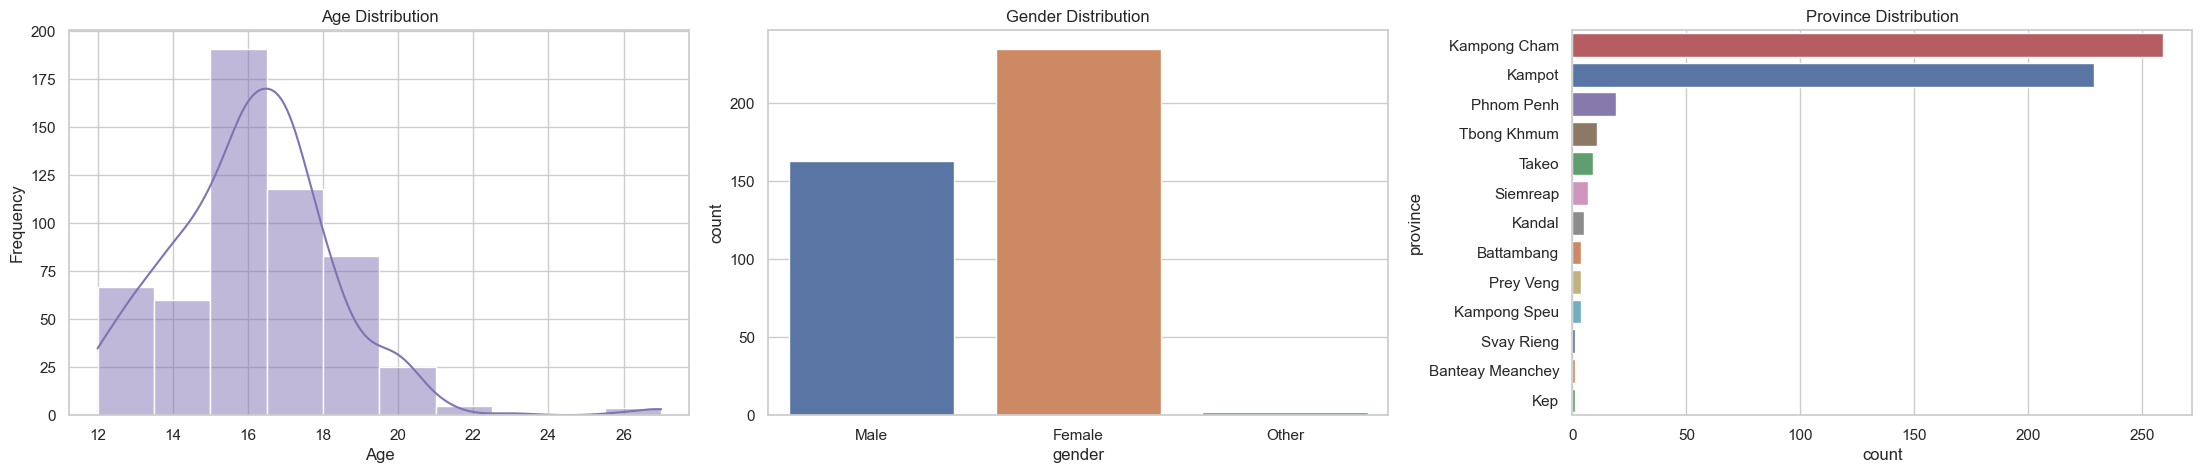
\includegraphics[width=0.95\textwidth]{Images/univariate_demographics.png}
    \caption{Univariate distributions of student demographics: (left) age distribution with kernel density estimate (KDE), (center) gender distribution count, and (right) province of study count ($N=400$).}
    \label{fig:univariate_demographics}
\end{figure}

The demographic analysis reveals the following insights:
\begin{itemize}
    \item \textbf{Age Distribution}: The age of the students in the cleaned dataset ranges from 12 to 27 years, with a bell-shaped distribution centered in the 15--20 year range (mean age $\approx 17.2$ years). This represents the typical age bracket for lower and upper secondary school students in Cambodia, including over-age students who enrolled late due to family economic constraints or geographic remoteness.
    \item \textbf{Gender Distribution}: The sample exhibits a balanced gender representation, with female students representing slightly more than half of the cohort. This balanced split ensures that gender-specific patterns are not statistically overshadowed in predictive modeling.
    \item \textbf{Province of Study}: The geographic distribution shows that the dataset is highly concentrated, with Kampong Cham and Kampot provinces jointly contributing approximately 90\% of the student responses. This concentration reflects the geographic focus of the rural data collection campaign, capturing cohorts from provinces characterized by high agricultural activity and seasonal labor demands.
\end{itemize}

\subsection{Univariate Academic Engagement and Performance Analysis}
\label{subsec:univariate_academic}

Student disengagement and academic struggle are key behavioral precursors to formal dropout. Figure~\ref{fig:univariate_disengagement} displays the frequency distributions of weekly attendance days, absence frequency, and average monthly study score level.

\begin{figure}[!ht]
    \centering
    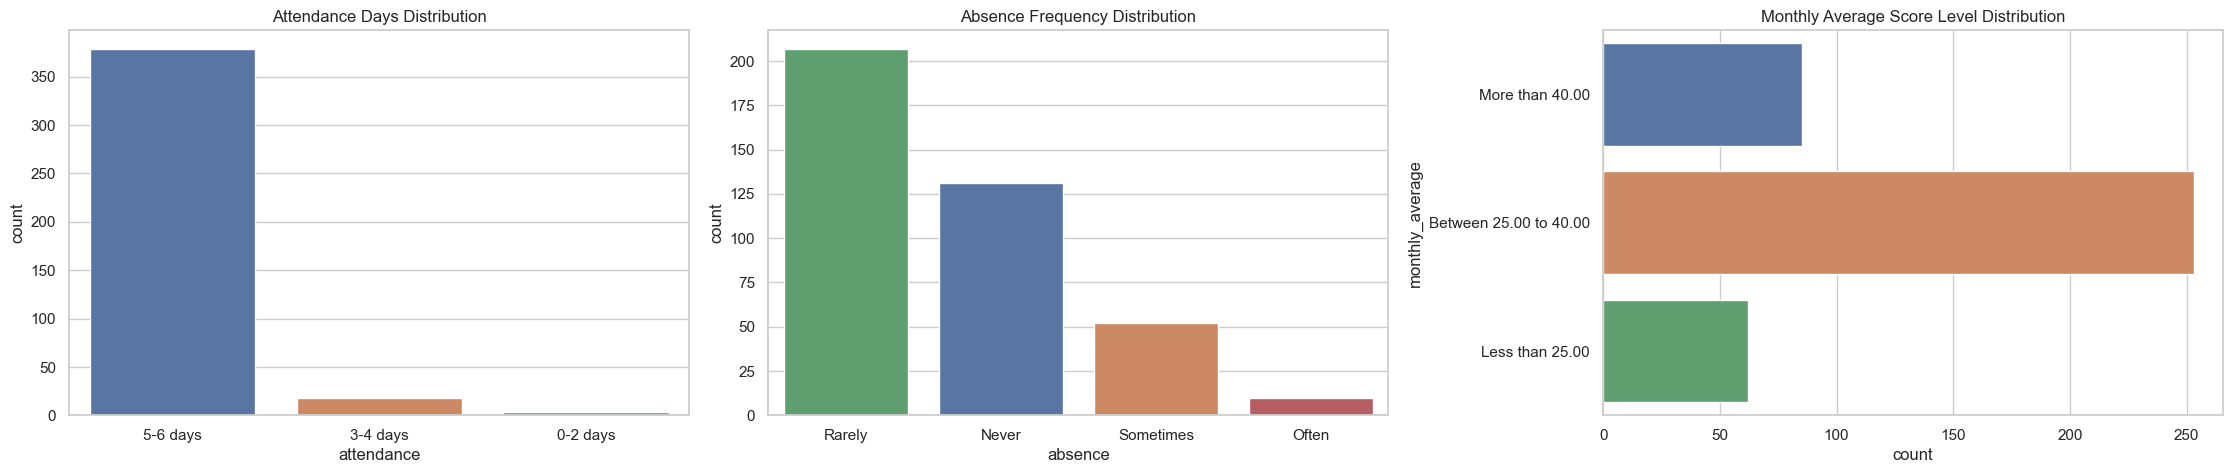
\includegraphics[width=0.95\textwidth]{Images/univariate_disengagement.png}
    \caption{Univariate distributions of academic disengagement and performance indicators: (left) weekly attendance days, (center) absence frequency, and (right) average monthly study score level ($N=400$).}
    \label{fig:univariate_disengagement}
\end{figure}

The academic profile shows:
\begin{itemize}
    \item \textbf{Weekly Attendance}: A large majority of students report high attendance regularity, attending school 5--6 days per week. However, a small but notable tail of students attend only 0--2 days or 3--4 days per week, signaling early-stage disengagement.
    \item \textbf{Absence Frequency}: Most students report "Never" or "Rarely" missing school days during a typical month. However, approximately 20\% of the sample reports missing school "Sometimes" or "Often", representing a group of students accumulating learning gaps.
    \item \textbf{Monthly Average Score}: Monthly academic averages are concentrated in the middle performance tier (score bracket 25--40), with lower proportions of students in the failing bracket ($<$25) or the high-achieving bracket ($>$40). Academic struggle correlates with lower self-efficacy, a critical driver of dropout thoughts.
\end{itemize}

\subsection{Univariate Socioeconomic and Support Environment Analysis}
\label{subsec:univariate_socioeconomics}

Household economic status and the strength of the immediate support environment are vital external factors in student retention. Figure~\ref{fig:univariate_socioeconomics} visualizes the distributions of parental education, living arrangements, student work support, and access to external NGO/scholarship aid.

\begin{figure}[!ht]
    \centering
    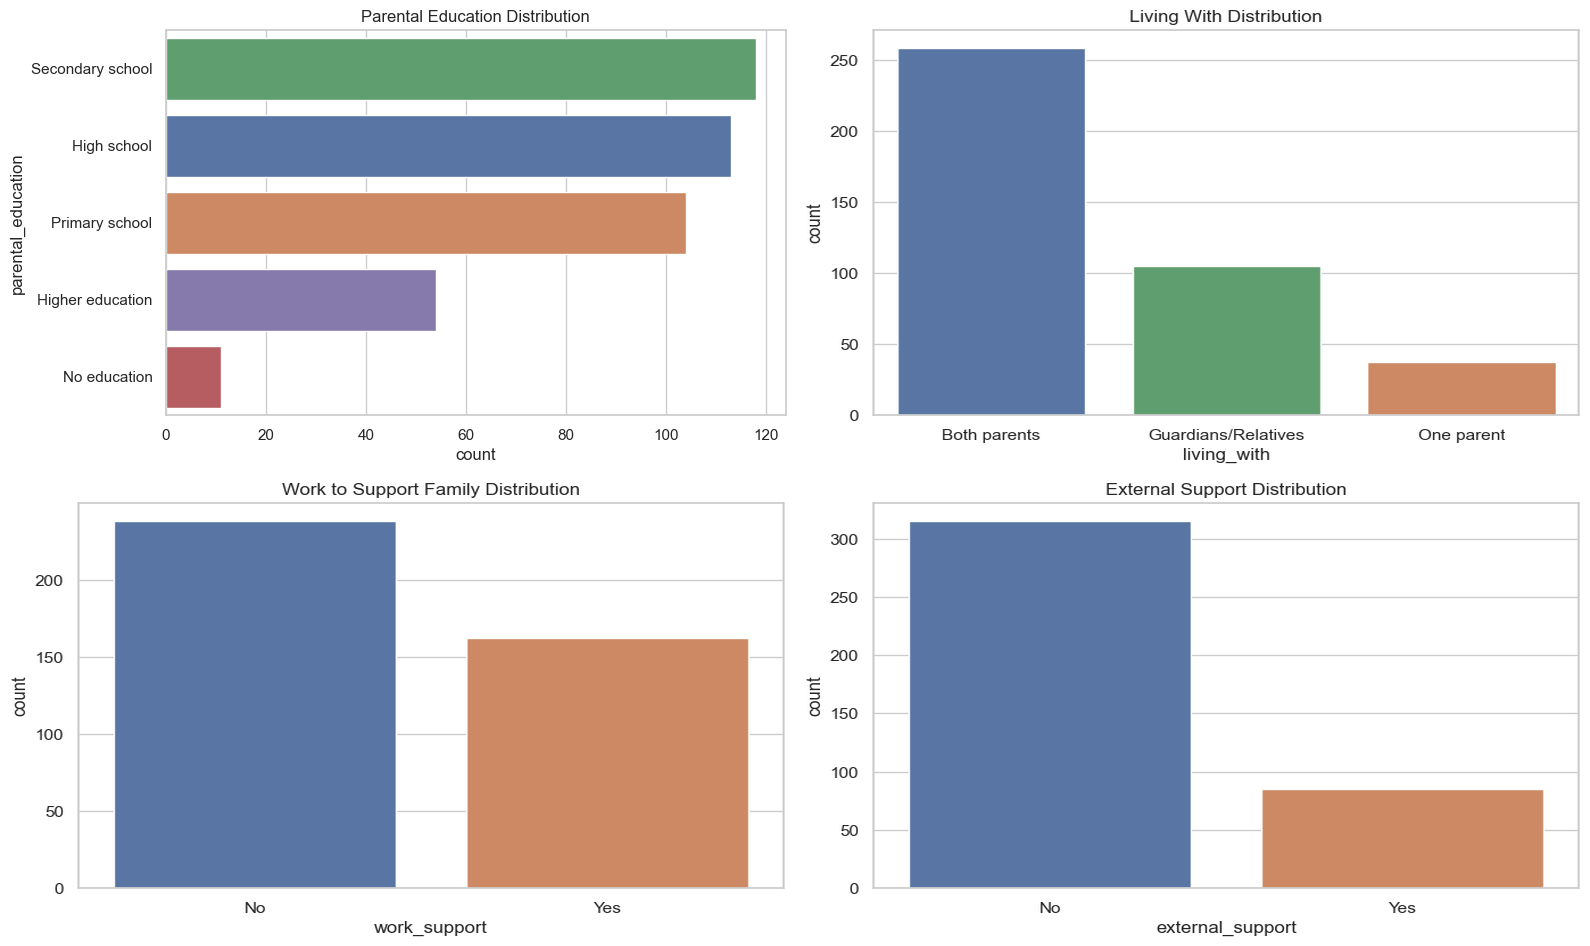
\includegraphics[width=0.9\textwidth]{Images/univariate_socioeconomics.png}
    \caption{Socioeconomic and support environment distributions: (top left) parental education level, (top right) living arrangements, (bottom left) student work-to-support-family status, and (bottom right) external NGO/scholarship support ($N=400$).}
    \label{fig:univariate_socioeconomics}
\end{figure}

The socioeconomic distributions indicate:
\begin{itemize}
    \item \textbf{Parental Education}: A significant majority of students report that their parents attained only primary school or high school education, with a very small percentage reporting tertiary or higher educational qualifications. Low parental educational attainment limits the household's capacity to provide academic homework guidance and resource support.
    \item \textbf{Living Situation}: Approximately 64\% of students live with both parents during the school term. However, a substantial minority live with single parents, grandparents, or relatives/guardians. In Cambodia, parental migration to urban centers (Phnom Penh) or neighboring countries (Thailand) for seasonal labor often results in students being left in the care of elderly grandparents, which reduces immediate household academic supervision.
    \item \textbf{Student Labor}: Approximately 24\% of students report having to work to support their family's income. Engaging in agricultural labor (especially during harvest seasons) or micro-business activities introduces severe time constraints, leading to chronic fatigue and high absence rates.
    \item \textbf{External Support}: Access to external financial or material support (such as NGO scholarships, bicycle donations, or school feeding programs) is reported by only 12\% of the cohort. This highlights the limited reach of formal support networks in the studied rural districts.
\end{itemize}

\subsection{Univariate Commute Burden Analysis}
\label{subsec:univariate_commute}

In rural Cambodia, infrastructure limitations pose physical barriers to school access. Figure~\ref{fig:univariate_commute} presents the distributions of distance from home to school and the primary transportation mode used by students.

\begin{figure}[!ht]
    \centering
    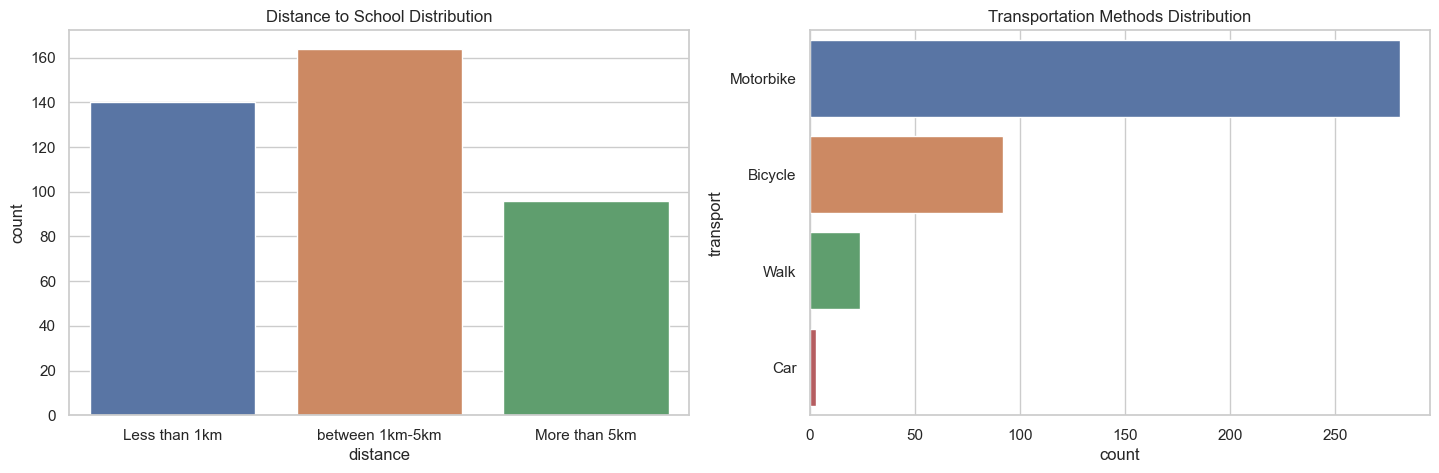
\includegraphics[width=0.95\textwidth]{Images/univariate_commute.png}
    \caption{Commute burden distributions: (left) distance from home to school, and (right) primary transportation mode used by students ($N=400$).}
    \label{fig:univariate_commute}
\end{figure}

The commute profiles show:
\begin{itemize}
    \item \textbf{Distance to School}: While the majority of students reside within 1--5\,km of their school, a significant subset (approximately 18\%) live more than 5\,km away. Long travel distances are highly critical in rural areas, where road quality is poor and seasonal flooding during the monsoon season can render roads impassable.
    \item \textbf{Transportation Mode}: Motorbike is the most common transport method, followed by bicycles and walking. Students who rely on walking or cycling for long commutes face increased physical strain, safety concerns, and vulnerability to weather conditions, directly compounding their risk of school disengagement.
\end{itemize}

\subsection{Univariate Target Variable Analysis}
\label{subsec:univariate_target}

For the target variable (\texttt{thought\_dropout}), Figure~\ref{fig:target_distribution} displays the class distribution count plot.

\begin{figure}[!ht]
    \centering
    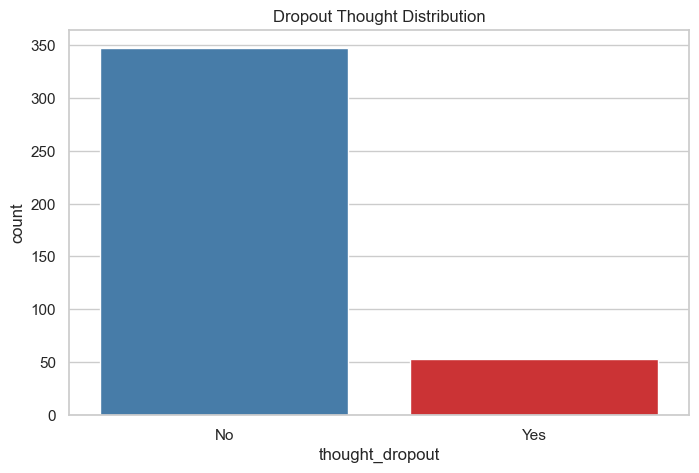
\includegraphics[width=0.55\textwidth]{Images/target_distribution.png}
    \caption{Target variable (\texttt{thought\_dropout}) class distribution, showing severe class imbalance ($N=400$; 347 non-at-risk vs.\ 53 at-risk students).}
    \label{fig:target_distribution}
\end{figure}

The target distribution reveals a \textbf{severe class imbalance}: only 53 students (13.25\%) reported having thoughts of dropping out of school, while 347 students (86.75\%) reported no dropout intentions. In machine learning, training classifiers on such skewed datasets without resampling causes models to default to majority-class predictions. This baseline imbalance necessitates the integration of synthetic oversampling techniques (such as SMOTE) in the modeling pipeline.

\subsection{Bivariate Analysis of Key Academic and Economic Risk Drivers}
\label{subsec:bivariate_academic_economic}

Bivariate analysis was conducted to examine the statistical patterns of survey features when stratified by the binary target variable (\texttt{thought\_dropout}). Figure~\ref{fig:bivariate_key_factors} presents bivariate count plots cross-tabulating weekly attendance, absence frequency, family income, and work support status against dropout thoughts.

\begin{figure}[!ht]
    \centering
    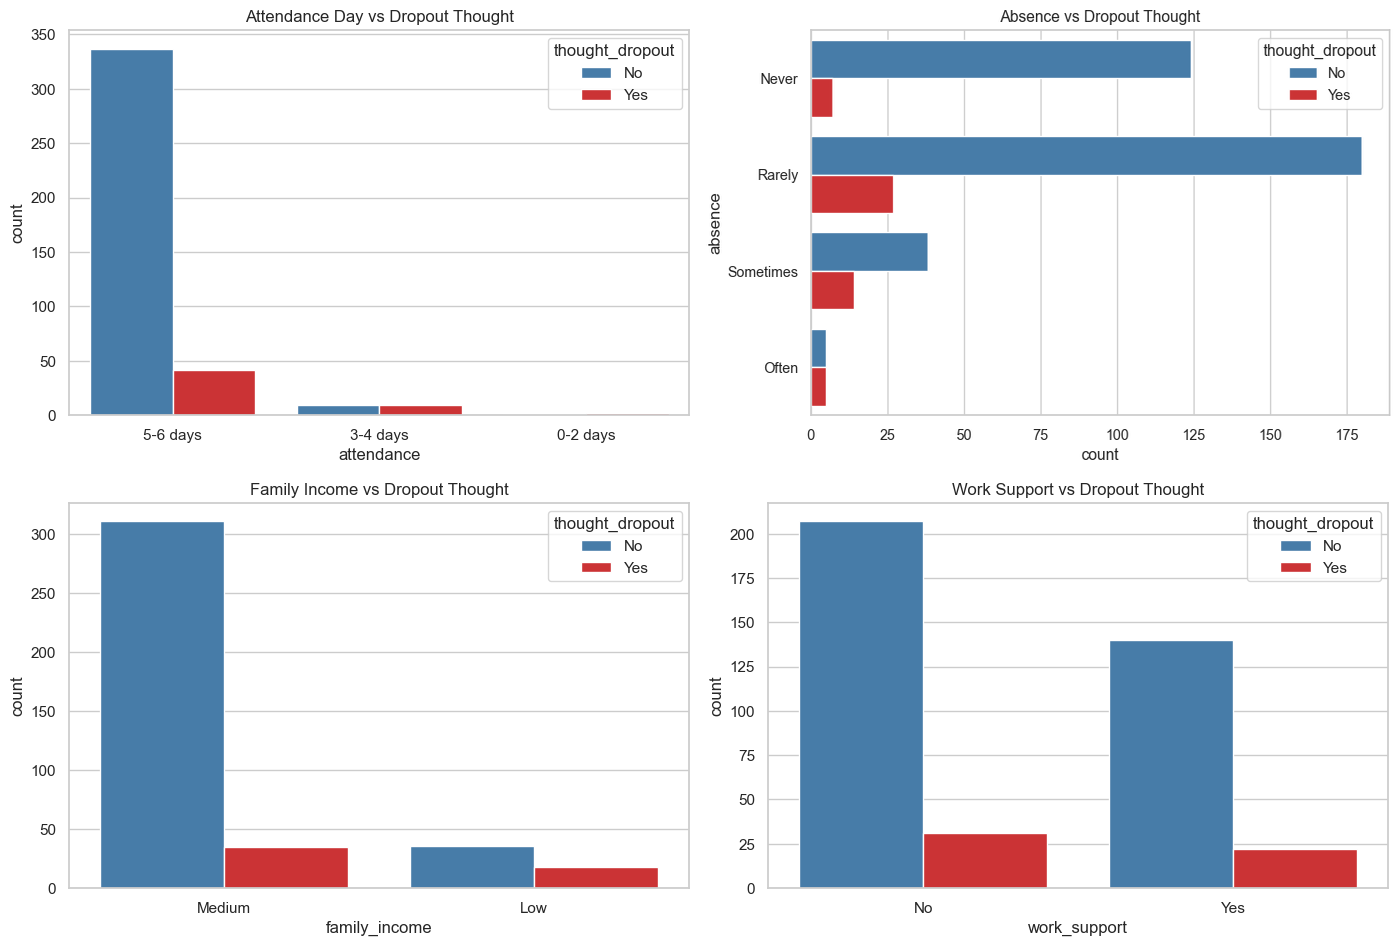
\includegraphics[width=0.95\textwidth]{Images/bivariate_key_factors.png}
    \caption{Bivariate count plots of key risk drivers vs.\ dropout thoughts: (a)~weekly attendance days, (b)~absence frequency, (c)~subjective family income level, and (d)~work-to-support-family status, stratified by the \texttt{thought\_dropout} class label.}
    \label{fig:bivariate_key_factors}
\end{figure}

Stratifying these key drivers reveals clear patterns:
\begin{itemize}
    \item \textbf{Weekly Attendance}: Students attending school only 0--2 days or 3--4 days per week exhibit a significantly higher proportion of dropout thoughts compared to those attending 5--6 days. Truancy is a strong behavioral indicator of active dropout risk.
    \item \textbf{Absence Frequency}: A clear gradient is visible: as absence frequency shifts from "Never" to "Often", the proportion of at-risk students rises dramatically. Frequent absences disrupt learning continuity, leading to low academic self-efficacy and eventual withdrawal.
    \item \textbf{Family Income}: Low-income students exhibit a higher rate of dropout thoughts compared to those from medium-income households. Household economic constraints represent a primary push factor, forcing students to choose between immediate labor earnings and long-term education.
    \item \textbf{Work Support}: Students who actively work to support their family show a larger proportion of dropout thoughts compared to those who do not work. This confirms that student labor competes directly with academic engagement.
\end{itemize}

\subsection{Bivariate Analysis of Contextual and Social Risk Drivers}
\label{subsec:bivariate_contextual_social}

Contextual and social factors, such as travel distance, transportation modes, family support, and parental education, also influence student attrition. Figure~\ref{fig:bivariate_contextual_factors} cross-tabulates these four contextual features against student dropout thoughts.

\begin{figure}[!ht]
    \centering
    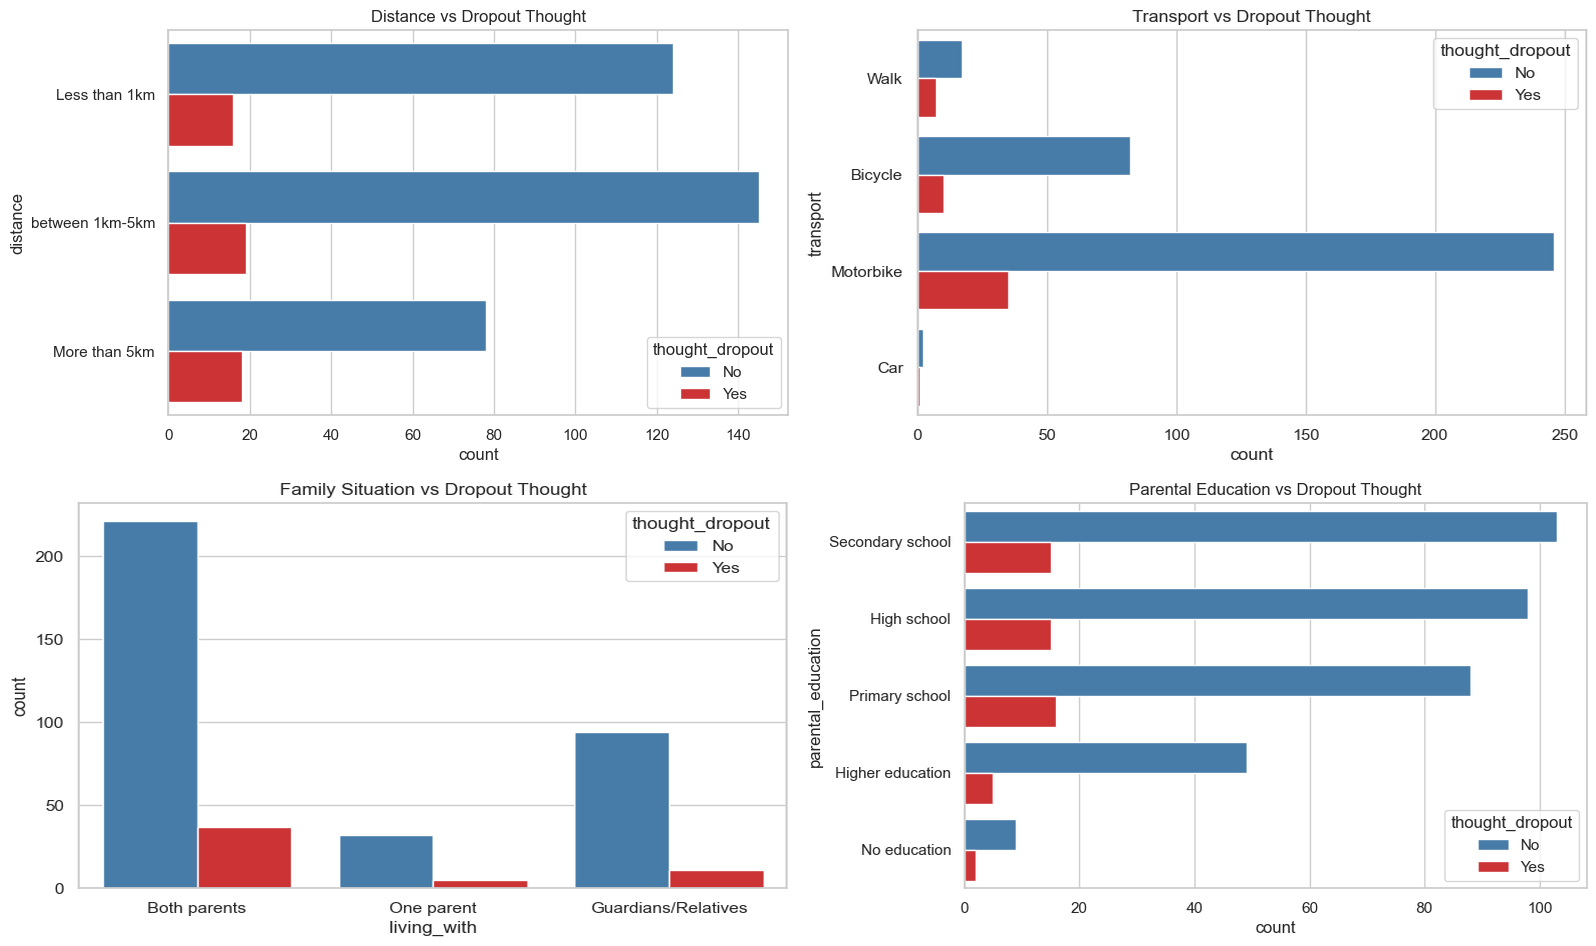
\includegraphics[width=0.95\textwidth]{Images/bivariate_contextual_factors.png}
    \caption{Bivariate count plots of contextual factors vs.\ dropout thoughts: (a)~distance to school, (b)~transportation mode, (c)~living situation, and (d)~parental education level, stratified by the \texttt{thought\_dropout} class label.}
    \label{fig:bivariate_contextual_factors}
\end{figure}

The bivariate analysis of these contextual factors reveals:
\begin{itemize}
    \item \textbf{Distance to School}: Students living more than 5\,km away from school exhibit a higher proportion of dropout thoughts compared to those living closer. This validates distance as a physical constraint on regular attendance.
    \item \textbf{Transportation Mode}: Students who walk or cycle to school show a higher relative proportion of dropout thoughts compared to those who ride motorbikes or travel by car, reflecting the increased physical strain of long commutes.
    \item \textbf{Living Situation}: Students living with a single parent, grandparents, or relatives/guardians have a notably higher dropout thought rate than those living with both parents. This supports the hypothesis that parental migration and the subsequent lack of parental supervision in the household elevate student vulnerability.
    \item \textbf{Parental Education}: Students whose parents have no formal education or only primary school attainment exhibit higher rates of dropout thoughts, indicating that household literacy levels are crucial buffers for academic perseverance.
\end{itemize}

\subsection{Correlation and Association Analysis}
\label{subsec:correlation}

A Pearson correlation heatmap was computed across all encoded features as a preliminary scan. Attendance frequency showed a moderate negative correlation with absence frequency ($r = -0.18$), and family income showed a weak negative correlation with work-to-support-family status ($r = -0.13$), indicating logical consistency in the dataset. However, because Pearson and Spearman correlation coefficients assume continuous or at minimum ordinal data and are technically invalid for nominal categorical variables, the study additionally computed bias-corrected \textbf{Cram\'{e}r's V} coefficients to quantify the true strength of association between each categorical survey variable and the binary dropout target.

The Cram\'{e}r's V coefficient between two nominal variables is mathematically formulated as:
\begin{equation}
    V = \sqrt{\frac{\chi^2 / n}{\min(k - 1,\; r - 1)}}
    \label{eq:cramers_v}
\end{equation}
where $\chi^2$ is the Pearson chi-square test statistic, $n$ is the total sample size, $k$ is the number of columns in the contingency table, and $r$ is the number of rows. A bias-correction term is applied to $\chi^2$ to account for small-sample inflation. The resulting Cram\'{e}r's V heatmap is displayed in Fig.~\ref{fig:cramers_v_heatmap}, and the exact ranked coefficients are detailed in Table~\ref{tab:cramers_v_coefficients}.

\begin{figure}[htbp]
    \centering
    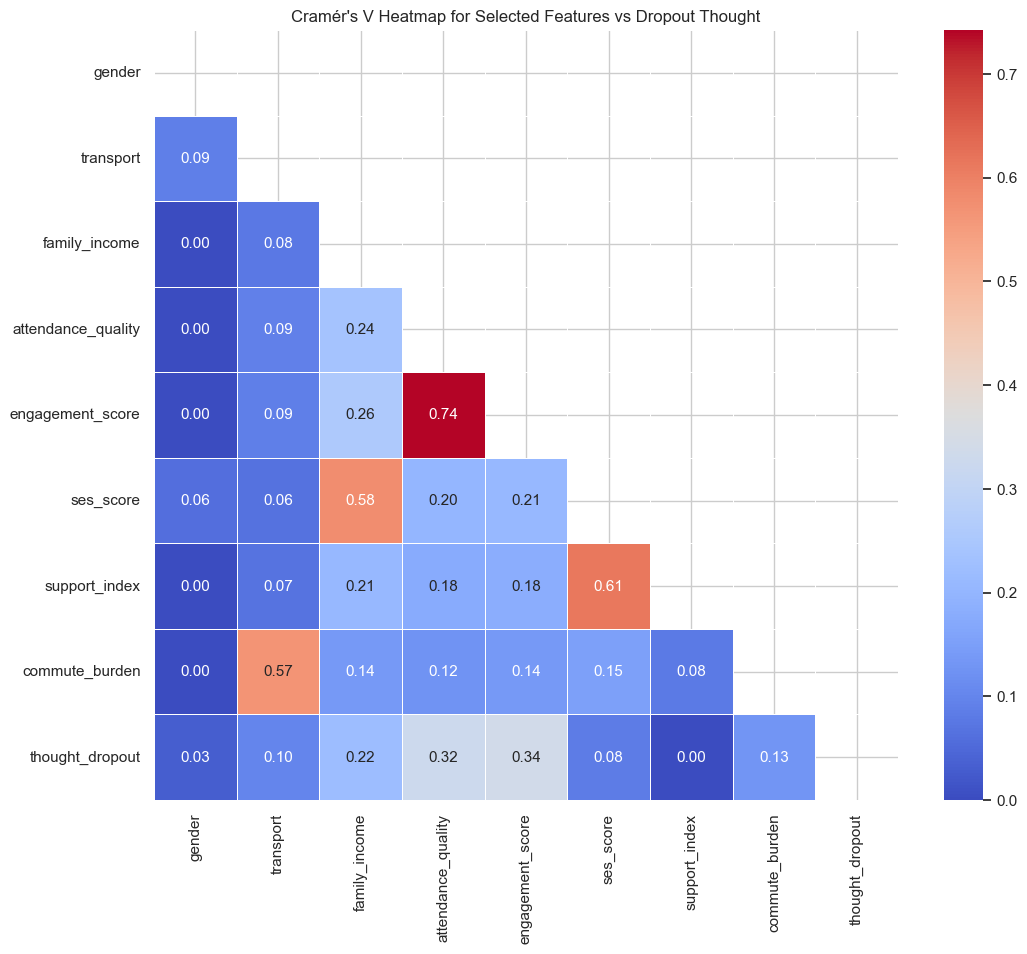
\includegraphics[width=0.85\textwidth]{Images/cramers_v_heatmap.png}
    \caption{Cram\'{e}r's V association heatmap displaying pairwise categorical association strengths across all survey features; columns/rows sorted by association strength with \texttt{thought\_dropout}.}
    \label{fig:cramers_v_heatmap}
\end{figure}

\begin{table}[htbp]
    \centering
    \caption{Ranked Cram\'{e}r's V Associations with Dropout Intention (\texttt{thought\_dropout})}
    \label{tab:cramers_v_coefficients}
    \begin{tabular}{clcc}
        \toprule
        \textbf{Rank} & \textbf{Survey Feature} & \textbf{Unadjusted Cram\'{e}r's V} & \textbf{Bias-Corrected Cram\'{e}r's V} \\
        \midrule
        1  & Weekly attendance days (\texttt{attendance})        & 0.2745 & 0.2656 \\
        2  & Absence frequency (\texttt{absence})                & 0.2614 & 0.2469 \\
        3  & Subjective family income (\texttt{family\_income})  & 0.2232 & 0.2178 \\
        4  & Monthly score average (\texttt{monthly\_average})   & 0.1591 & 0.1427 \\
        5  & Living arrangements (\texttt{living\_with})         & 0.1358 & 0.1047 \\
        6  & Primary transport mode (\texttt{transport})         & 0.1318 & 0.0994 \\
        7  & Distance to school (\texttt{distance})              & 0.0912 & 0.0575 \\
        8  & Student gender (\texttt{gender})                    & 0.0776 & 0.0317 \\
        9  & Parental education (\texttt{parental\_education})   & 0.0596 & 0.0000 \\
        10 & External NGO/scholarship aid (\texttt{external\_support}) & 0.0318 & 0.0000 \\
        11 & Works to support family (\texttt{work\_support})    & 0.0005 & 0.0000 \\
        \bottomrule
    \end{tabular}
\\ \medskip
\raggedright \footnotesize \textbf{Note on Zero Associations}: Several contextual features (parental education, external support, and student work support) yield a bias-corrected Cram\'{e}r's V of exactly $0.0000$. This occurs due to the Bergsma bias-correction penalty term $\frac{(k-1)(r-1)}{n-1}$ exceeding the raw phi-squared value ($\chi^2/n$) for weakly associated features. Showing both unadjusted and bias-corrected coefficients demonstrates that while these variables have weak raw associations (e.g., $0.0596$ for parental education), their standalone predictive power is statistically negligible. This justifies the necessity of aggregating them into composite engineered features.
\end{table}

The association analysis reveals that school disengagement metrics (attendance quality and absence frequency) and household socioeconomic status (family income) are the three strongest individual statistical predictors of dropout intention. As noted in Table~\ref{tab:cramers_v_coefficients}, several individual variables yield a bias-corrected Cram\'{e}r's V of exactly $0.0000$ due to the Bergsma penalty term capping weak associations at zero. For student labor support (\texttt{work\_support}), the unadjusted association is virtually zero ($0.0005$), as both working and non-working students exhibit almost identical dropout thought rates in the raw survey data (13.6\% vs. 13.0\%, respectively). Consequently, while these individual factors are contextually important, they carry negligible standalone predictive power and must be combined into composite engineered features to expose their combined predictive signals.

%%============================================================================
\section{Feature Engineering}
\label{sec:feature_engineering}

To improve model performance and create more informative representations of student vulnerability, six composite features were engineered from the raw survey variables. The engineering decisions were guided by domain knowledge from the literature review---specifically the IAFREE relational model by Vasconcelos et al.\ (2023) and Cambodia-specific educational risk drivers documented by Kreng et al.\ (2016)---and by patterns observed in the EDA, particularly the finding that several individually weak features (parental education, external support, work support) carry no individual predictive power and must be aggregated to become useful.

Table~\ref{tab:feature_engineering_table} presents the full set of engineered features with their mathematical formulations and theoretical rationale.

\begin{longtable}{|p{2.8cm}|p{5.0cm}|p{7.8cm}|}
    \caption{Engineered Composite Features and Their Formulations}
    \label{tab:feature_engineering_table} \\
    \hline
    \rowcolor{gray!20}
    \textbf{Feature Name} &
    \textbf{Formula} &
    \textbf{Rationale} \\
    \hline
    \endfirsthead

    \multicolumn{3}{c}{\tablename~\thetable{} -- continued from previous page} \\
    \hline
    \rowcolor{gray!20}
    \textbf{Feature Name} &
    \textbf{Formula} &
    \textbf{Rationale} \\
    \hline
    \endhead

    \hline \multicolumn{3}{r}{\textit{Continued on next page}} \\
    \endfoot

    \hline
    \endlastfoot

    \textbf{Attendance Quality ($AQ$)} &
    $AQ = x_{\text{attendance}} - x_{\text{absence}}$ &
    Captures the \textit{net quality} of school attendance by subtracting absence frequency from attendance regularity, yielding a single signed score that reflects both engagement and disruption simultaneously. A negative value signals chronic truancy. \\
    \hline

    \textbf{Engagement Score ($ES$)} &
    $ES = x_{\text{attendance}} + x_{\text{monthly\_average}} - x_{\text{absence}}$ &
    Extends Attendance Quality by incorporating academic performance, producing a holistic metric of active academic participation. Students with high attendance and strong scores but few absences receive high $ES$ values. \\
    \hline

    \textbf{SES Score ($SES$)} &
    \parbox{4.8cm}{\vspace{0.1cm}\raggedright $SES = x_{\text{family\_income}} +$\\ $x_{\text{parental\_education}} +$\\ $x_{\text{external\_support}}$\vspace{0.1cm}} &
    Aggregates household financial capacity, parental intellectual capital, and access to external aid into a single composite index of socioeconomic status. Individually these features have near-zero Cram\'{e}r's V, but combined they differentiate economic vulnerability. \\
    \hline

    \textbf{Support Index ($SI$)} &
    \parbox{4.8cm}{\vspace{0.1cm}\raggedright $SI = x_{\text{living\_with}} +$\\ $x_{\text{external\_support}} +$\\ $x_{\text{parental\_education}}$\vspace{0.1cm}} &
    Measures the strength of the student's \textit{protective environment} from family structure and institutional support networks. Captures both direct household supervision and indirect support channels. \\
    \hline

    \textbf{Commute Burden ($CB$)} &
    $CB = x_{\text{distance}} + x_{\text{transport}}$ &
    Captures the physical and logistical difficulty of reaching school, representing the structural barriers to attendance in rural Cambodian infrastructure, where road quality and transport accessibility directly constrain school participation. \\
    \hline

    \textbf{Weighted Risk Score ($WRS$)} &
    \parbox{4.8cm}{\vspace{0.1cm}\raggedright $WRS = 0.3 \cdot x_{\text{absence}} +$\\ $0.1 \cdot x_{\text{work\_support}} +$\\ $0.2 \cdot x_{\text{distance}} +$\\ $0.4 \cdot y_{\text{thought\_dropout}}$\vspace{0.1cm}} &
    A composite risk index that weights three contextual indicators and the target variable itself ($y_{\text{thought\_dropout}}$). Because this feature explicitly incorporates the target variable, it is target-informed and would introduce severe target leakage if used in classification models. Therefore, it is excluded from prediction features and reserved solely for the unsupervised clustering stage to generate target-informed student profiles. \\
    \hline

\end{longtable}

Following feature construction, the engineered features were validated by computing their correlations with the target variable. The Engagement Score showed the strongest Pearson correlation with \texttt{thought\_dropout} ($r = -0.32$), confirming that the composite better captures dropout risk than any individual raw feature. The engineered correlation heatmap revealed high multicollinearity between Attendance Quality and Engagement Score ($r = 0.82$), and between SES Score and Support Index ($r = 0.91$), reflecting the intended design redundancy in these complementary pairs. These correlated features are retained for the unsupervised clustering stage to enrich cluster separation, but their multicollinearity is acknowledged as a potential concern for linear classifiers.

%%============================================================================
\section{Student Segmentation via K-Means Clustering}
\label{sec:student_segmentation}

To profile distinct student subgroups and understand vulnerability patterns beyond binary classification, an unsupervised K-Means clustering algorithm was applied to the standardized engineered features. This segmentation stage supplements the predictive model by providing interpretable student risk archetypes---Low Risk, Medium Risk, and High Risk groups---that can be visualized and filtered in the EWS dashboard.

The six engineered features ($AQ$, $ES$, $SES$, $SI$, $CB$, $WRS$) were standardized using Z-score normalization to ensure equal contribution to the Euclidean distance computation:
\begin{equation}
    z_i = \frac{x_i - \mu_i}{\sigma_i}
    \label{eq:zscore}
\end{equation}
where $\mu_i$ is the feature mean and $\sigma_i$ is the standard deviation across the dataset. The K-Means objective function minimizes the within-cluster sum of squared Euclidean distances (inertia):
\begin{equation}
    J = \sum_{j=1}^{k} \sum_{i \in C_j} \left\| z_i - \mu_j \right\|^2
    \label{eq:kmeans_inertia}
\end{equation}
where $C_j$ is the set of students assigned to cluster $j$ and $\mu_j$ is the centroid of cluster $j$. The algorithm iteratively updates cluster assignments and centroids until convergence.

\subsection{Optimal Cluster Selection Methodology}
\label{subsec:optimal_k_method}

The optimal number of clusters $k$ was determined by evaluating both the Elbow Method (inertia vs.\ $k$) and the Silhouette Score across $k \in \{2, 3, \ldots, 9\}$. The Silhouette Score for a given student $i$ is defined as:
\begin{equation}
    s(i) = \frac{b(i) - a(i)}{\max\{a(i),\; b(i)\}}
    \label{eq:silhouette}
\end{equation}
where $a(i)$ is the mean intra-cluster distance (cohesion) and $b(i)$ is the mean distance to the nearest neighboring cluster (separation). Values of $s(i)$ close to $+1$ indicate well-separated, compact clusters. The empirical evaluations of the Elbow Method and Silhouette Analysis are presented and discussed in Chapter 5.

\subsection{Cluster Visualization via PCA Projection}
\label{subsec:pca_clusters_method}

To visualize the 6-dimensional cluster boundaries in two dimensions, Principal Component Analysis (PCA) was applied to project the standardized feature space onto the first two principal components (PC1 and PC2). PCA finds orthogonal directions of maximum variance, with the first principal component $\mathbf{p}_1$ defined as:
\begin{equation}
    \mathbf{p}_1 = \underset{\|\mathbf{w}\| = 1}{\arg\max}\; \mathrm{Var}\left(\mathbf{Z}\,\mathbf{w}\right)
    \label{eq:pca}
\end{equation}
where $\mathbf{Z}$ is the standardized data matrix. The projected 2D visualization of the clusters is detailed in Chapter 5.

\subsection{Cluster Profiling and Risk Label Assignment}
\label{subsec:cluster_profiling_method}

To interpret and label each cluster, the feature means and outcomes (actual dropout thoughts and high-risk flags) were analyzed within each cluster. The resulting cluster profiles, risk assignments, and characterizations are fully detailed in Chapter 5.

%%============================================================================
\section{Predictive Modelling}
\label{sec:predictive_modelling}

\subsection{Problem Formulation and Evaluation Metrics}
\label{subsec:eval_metrics}

The predictive modelling task is a binary classification problem: given a student's engineered feature vector $\mathbf{x} \in \mathbb{R}^{5}$, predict whether the student has thought about dropping out ($y = 1$) or not ($y = 0$). The five engineered features used as predictors are Attendance Quality ($AQ$), Engagement Score ($ES$), SES Score ($SES$), Support Index ($SI$), and Commute Burden ($CB$). The Weighted Risk Score ($WRS$) is deliberately excluded from the supervised prediction pipeline because it was constructed to incorporate contextual risk weights and is reserved exclusively for the unsupervised clustering stage described in Section~\ref{sec:student_segmentation}, preventing any form of target-proxy leakage. Given the significant class imbalance in the dataset (86.75\% negative, 13.25\% positive), model selection was guided primarily by the \textbf{Recall} and \textbf{F1-Score} on the minority class, because the societal cost of a False Negative---missing a student who is genuinely at risk---is substantially greater than the cost of a False Positive in an educational intervention context. The five primary evaluation metrics used are defined as follows:

\begin{equation}
    \text{Accuracy} = \frac{TP + TN}{TP + TN + FP + FN}
    \label{eq:accuracy}
\end{equation}

\begin{equation}
    \text{Recall (Sensitivity)} = \frac{TP}{TP + FN}
    \label{eq:recall}
\end{equation}

\begin{equation}
    \text{Precision} = \frac{TP}{TP + FP}
    \label{eq:precision}
\end{equation}

\begin{equation}
    \text{F1-Score} = 2 \times \frac{\text{Precision} \times \text{Recall}}{\text{Precision} + \text{Recall}}
    \label{eq:f1}
\end{equation}

where $TP$, $TN$, $FP$, and $FN$ denote True Positives, True Negatives, False Positives, and False Negatives, respectively. Additionally, the Area Under the Receiver Operating Characteristic Curve (ROC-AUC) was computed as a threshold-independent measure of discriminative capability.

\subsection{Class Imbalance and Resampling Strategies}
\label{subsec:resampling}

Given the 86.75\%\,/\,13.25\% class split in the training data ($N_{\text{train}}=256$), six resampling strategies were applied to the training set to mitigate bias toward majority-class predictions. Their resulting training-set class distributions are visualized in Fig.~\ref{fig:resampling_distributions}:
\begin{itemize}
    \item \textbf{Original} (no resampling) --- class-weighted baseline using \texttt{class\_weight=`balanced'}
    \item \textbf{SMOTE} (Synthetic Minority Oversampling Technique) --- generates synthetic at-risk instances by linear interpolation between minority-class neighbors
    \item \textbf{ADASYN} (Adaptive Synthetic Sampling) --- focuses synthetic generation on harder-to-classify minority boundary samples
    \item \textbf{RandomUnderSampler} --- randomly removes majority-class samples to achieve class balance
    \item \textbf{SMOTE-Tomek} --- SMOTE oversampling followed by Tomek-link removal to clean borderline majority instances
    \item \textbf{SMOTE-ENN} --- SMOTE oversampling followed by Edited Nearest Neighbors (ENN) cleaning to remove noisy boundary samples
\end{itemize}

The SMOTE algorithm generates a synthetic minority instance $x_{\text{new}}$ by interpolating between a minority instance $x_i$ and one of its $k$-nearest minority neighbors $x_{zi}$:
\begin{equation}
    x_{\text{new}} = x_i + \lambda \left(x_{zi} - x_i\right), \quad \lambda \sim U(0,\,1)
    \label{eq:smote}
\end{equation}
where $\lambda$ is drawn uniformly from $[0, 1]$. All resampling was applied exclusively within each training fold of the cross-validation pipeline to prevent data leakage into the validation or test partitions.

\begin{figure}[!ht]
    \centering
    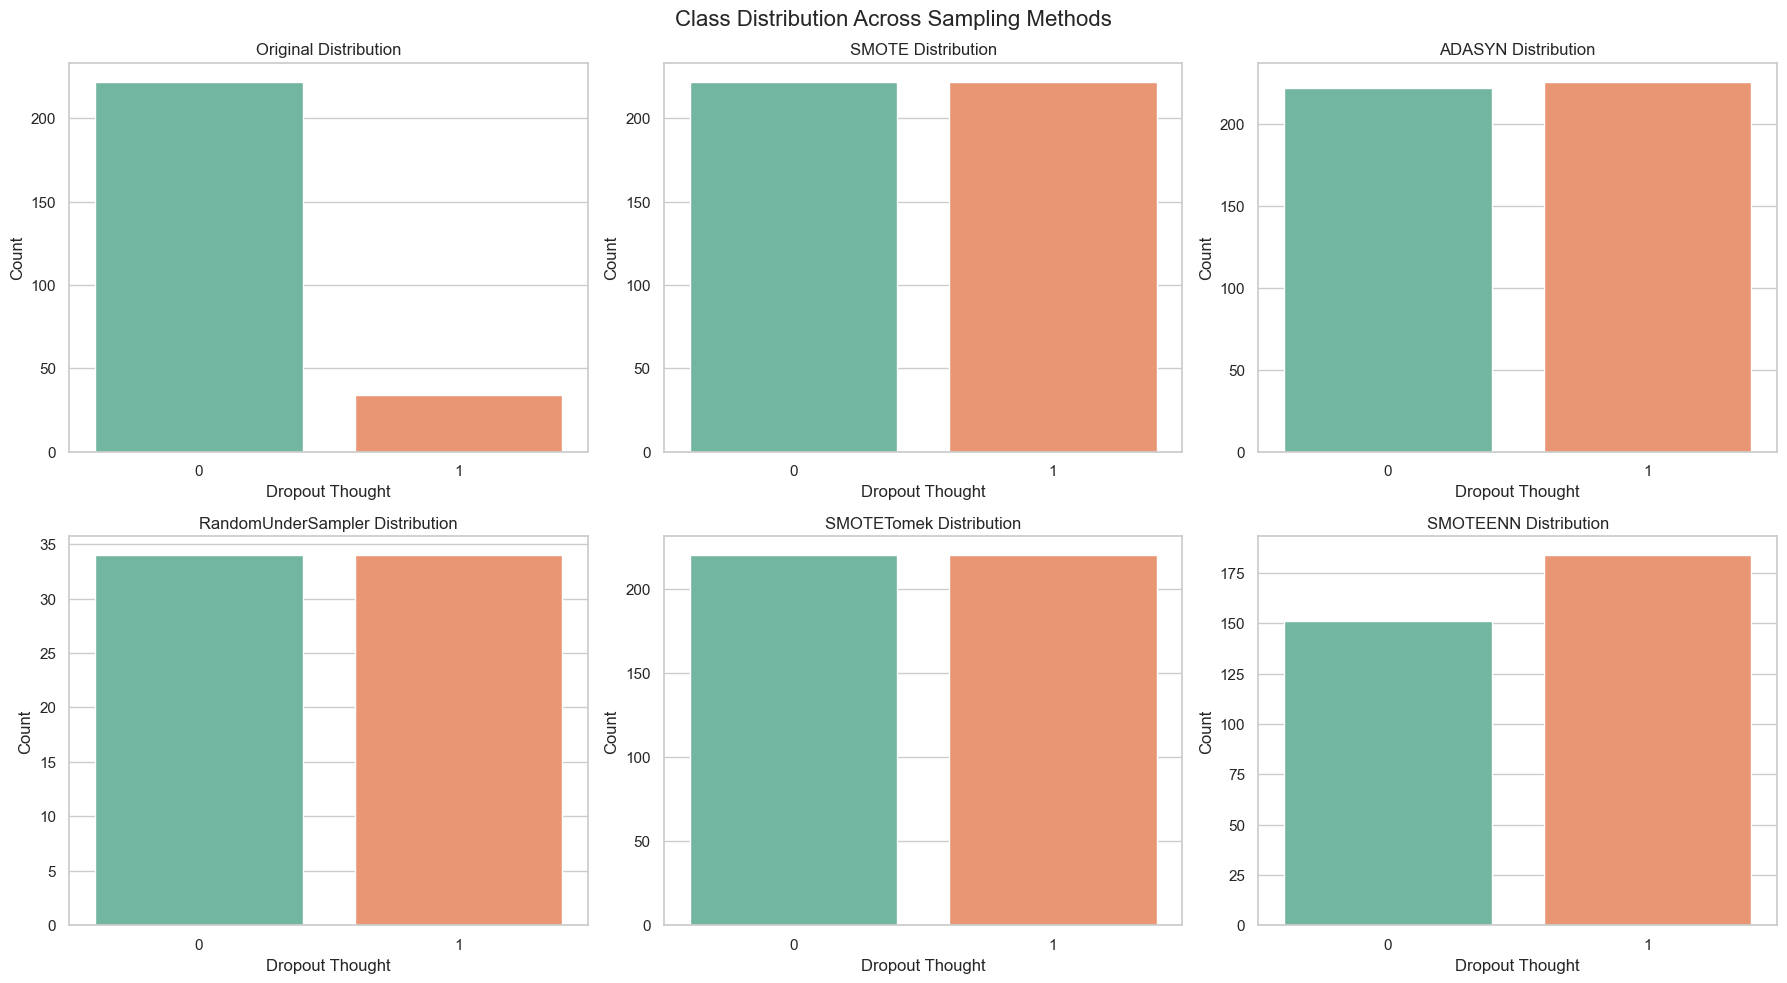
\includegraphics[width=\textwidth]{Images/resampling_distributions.png}
    \caption{Training-set class distributions under six resampling strategies, showing the degree of minority class oversampling or majority class undersampling applied in each configuration.}
    \label{fig:resampling_distributions}
\end{figure}

\subsection{Classifiers Evaluated}
\label{subsec:classifiers}

Eight classifiers were evaluated across all six resampling strategies, covering a range of algorithm families from linear models to ensemble methods. Table~\ref{tab:classifiers_table} lists each classifier with its theoretical rationale for inclusion.

\begin{longtable}{|p{4.2cm}|p{11.4cm}|}
    \caption{Classification Algorithms Evaluated in the EWS Pipeline}
    \label{tab:classifiers_table} \\
    \hline
    \rowcolor{gray!20}
    \textbf{Classifier} &
    \textbf{Rationale for Inclusion} \\
    \hline
    \endfirsthead

    \multicolumn{2}{c}{\tablename~\thetable{} -- continued from previous page} \\
    \hline
    \rowcolor{gray!20}
    \textbf{Classifier} &
    \textbf{Rationale for Inclusion} \\
    \hline
    \endhead

    \hline \multicolumn{2}{r}{\textit{Continued on next page}} \\
    \endfoot

    \hline
    \endlastfoot

    \textbf{Logistic Regression (LR)} &
    Simple, interpretable linear baseline. Provides probability outputs natively, making it suitable for threshold tuning. Well-suited to linearly separable feature spaces. \\
    \hline

    \textbf{Support Vector Machine (SVM)} &
    Effective in high-dimensional, low-sample settings. The kernel trick (RBF kernel) allows non-linear decision boundaries. The maximum-margin hyperplane is robust to class overlap in low-density minority regions. \\
    \hline

    \textbf{Decision Tree (DT)} &
    Non-parametric, inherently interpretable. Serves as a baseline for all tree-based ensemble methods and exposes axis-aligned split logic for counsellor interpretability. \\
    \hline

    \textbf{Random Forest (RF)} &
    Ensemble of decorrelated decision trees trained via bagging. Robust to overfitting in high-variance settings; provides feature importance rankings. \\
    \hline

    \textbf{Extra Trees} &
    Extremely Randomized Trees; introduces additional randomization in split-point selection, often yielding lower variance than Random Forest with competitive accuracy. \\
    \hline

    \textbf{Gradient Boosting (GB)} &
    Sequential residual-correction ensemble; each tree corrects the prediction errors of the prior ensemble. Strong on tabular imbalanced data when combined with class weighting. \\
    \hline

    \textbf{XGBoost} &
    Optimized, regularized implementation of gradient boosting with built-in L1/L2 penalties, missing-value handling, and fast convergence via second-order gradient approximation. \\
    \hline

    \textbf{LightGBM} &
    Histogram-based gradient boosting that grows trees leaf-wise rather than depth-wise. Highly efficient on datasets with many features; natively supports class-weight parameters. \\
    \hline

\end{longtable}

Additionally, a \textbf{Soft Voting Ensemble} was constructed by averaging the predicted class probabilities of four fixed base estimators---Logistic Regression, SVM, Random Forest, and XGBoost---each trained on SMOTE-resampled data. This ensemble was evaluated as a standalone configuration on the held-out test set for direct comparison against the selected SMOTE~+~SVM pipeline.

\subsection{Training Pipeline and Hyperparameter Tuning}
\label{subsec:pipeline}

Each classifier--resampler combination was encapsulated in a \texttt{scikit-learn} \texttt{Pipeline} object with the resampler placed \textit{inside} the cross-validation loop using a 5-fold \texttt{StratifiedKFold} strategy (\texttt{random\_state=42}). This architecture strictly prevents data leakage by ensuring that each resampler only observes the training fold during fitting, while the validation fold remains untouched. Models were first compared using direct validation-set evaluation across all 48 classifier--resampler combinations (8 classifiers $\times$ 6 samplers), followed by 5-fold stratified cross-validation to confirm that validation performance generalizes. Hyperparameter optimization for the final selected pipeline was performed using \texttt{RandomizedSearchCV} with F1-Score (minority class) as the scoring criterion, over \textbf{20 random parameter combinations} (\texttt{n\_iter=20}), with 5-fold stratified cross-validation.

The performance comparison of the classification models across the various resampling strategies, the hyperparameter tuning results, and the selection of the final prediction pipeline are detailed and discussed in Chapter 5.

\subsection{Decision Threshold Tuning}
\label{subsec:threshold}

To further improve Recall on the positive (at-risk) class, the default decision threshold of $\tau = 0.50$ was adjusted by sweeping threshold values from 0.10 to 0.95 in steps of 0.05 on the validation set ($N_{\text{val}}=64$). For each candidate threshold, Precision, Recall, and F1-Score were computed. The details of the threshold sweep, the resulting Precision-Recall-F1 curves, and the selection of the final operational classification threshold are presented and discussed in Chapter 5.

\subsection{Model Explainability via SHAP}
\label{subsec:shap}

To address the interpretability requirements of an EWS deployed in a school counselling context, SHAP (SHapley Additive exPlanations) values were computed for the final SMOTE~+~SVM model using a \texttt{KernelExplainer} applied to the scaled test set. SHAP is grounded in cooperative game theory: the Shapley value of feature $i$ for a single prediction is defined as:
\begin{equation}
    \phi_i(f) = \sum_{S \subseteq F \setminus \{i\}} \frac{|S|!\,(|F| - |S| - 1)!}{|F|!} \left[ f(S \cup \{i\}) - f(S) \right]
    \label{eq:shap}
\end{equation}
where $F$ is the full feature set ($|F|=5$), $S$ is any subset of features not containing $i$, and $f(S)$ is the model's expected output using only features in $S$. A positive SHAP value indicates that feature $i$ pushes the model's prediction toward dropout risk ($y=1$); a negative value pushes it toward non-risk ($y=0$). The SHAP beeswarm plot and per-student waterfall charts generated from this analysis are presented and discussed in Chapter~5 (Results and Discussion).

%%============================================================================
\section{UI Dashboard Development}
\label{sec:dashboard}

A web-based EWS dashboard was developed as the user-facing interface of the system, designed to be accessible to non-technical stakeholders---specifically school counsellors, teachers, and educational administrators. The dashboard was built using \textbf{React.js} as the front-end framework and \textbf{Tailwind CSS} for responsive layout and design. The backend API layer was implemented using \textbf{FastAPI} (Python), which exposes the trained SMOTE + SVM model as a REST prediction endpoint. Communication between the front-end and backend follows an asynchronous HTTP request pattern, enabling real-time risk scoring on submitted student survey data.

The dashboard comprises four primary interactive modules:
\begin{enumerate}
    \item \textbf{Student Risk Prediction:} A form-based interface that accepts a student's survey responses as input and calls the FastAPI prediction endpoint. The response includes a real-time dropout probability score, a risk tier label (Low / Medium / High), and per-feature SHAP waterfall values explaining the prediction in plain language.
    \item \textbf{Cluster Visualisation:} An interactive scatter plot (PCA projection) displaying all students grouped into their K-Means risk clusters. Counsellors can filter the visualisation by province, gender, grade level, and risk tier to identify at-risk subgroups for targeted intervention.
    \item \textbf{SHAP Explainability View:} Per-student SHAP waterfall charts decompose each individual risk score into its contributing feature factors, allowing counsellors to understand and communicate the reasoning behind each prediction in the context of the student's actual survey responses.
    \item \textbf{Analytics Dashboard:} Aggregated summary statistics including total enrolled students, current risk tier distribution (Low / Medium / High), attendance trends by grade, monthly at-risk counts, and a list of recent high-risk alerts are presented as interactive charts and data cards.
\end{enumerate}

At the time of submission, the dashboard prototype is operational with the trained SVM model integrated via the FastAPI endpoint. The system successfully processes survey input forms, returns real-time risk predictions, and renders SHAP explanations for individual students. Deployment to a production server and the integration of an authenticated multi-school data management layer are designated as future work.
